\documentclass[tikz]{standalone}

\usepackage{fontspec}

\usetikzlibrary{arrows}
\usetikzlibrary{calc}
\usetikzlibrary{decorations.pathreplacing}
\usetikzlibrary{positioning}
\usetikzlibrary{matrix}

\usepackage{fontspec}

\begin{document}

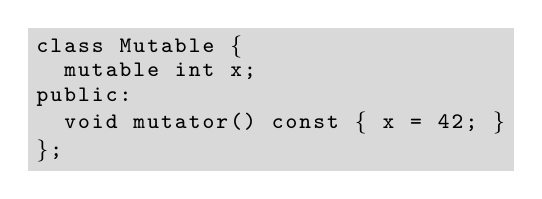
\begin{tikzpicture}
  [node distance=5mm, >=stealth',
  every node/.style={font=\footnotesize},
  every matrix/.style={fill=black!15, inner sep=1mm, row sep=0.5mm,
                        matrix of nodes, nodes in empty cells,
                        minimum height=0.5em, minimum width=.5em,
                        nodes={anchor=base, inner sep=0, font=\ttfamily\footnotesize}}]

  \matrix {
c & l & a & s & s &   & M & u & t & a & b & l & e &   & \{ &   &   &   &   &   &   &   &   &   &   &   &   &   &   &   &   &   &   &   \\
  &   & m & u & t & a & b & l & e &   & i & n & t &   & x & ; &   &   &   &   &   &   &   &   &   &   &   &   &   &   &   &   &   &   \\
p & u & b & l & i & c & : &   &   &   &   &   &   &   &   &   &   &   &   &   &   &   &   &   &   &   &   &   &   &   &   &   &   &   \\
  &   & v & o & i & d &   & m & u & t & a & t & o & r & ( & ) &   & c & o & n & s & t &   & \{ &   & x &   & = &   & 4 & 2 & ; &   & \} \\
\} & ; &   &   &   &   &   &   &   &   &   &   &   &   &   &   &   &   &   &   &   &   &   &   &   &   &   &   &   &   &   &   &   &   \\
  };
\end{tikzpicture}

\end{document}
